\documentclass[journal]{IEEEtran}
\usepackage{amsmath,amssymb}
\usepackage{graphicx}
\usepackage{booktabs}
\usepackage{cite}
\usepackage{url}
\usepackage[hidelinks]{hyperref}
% shrink a tabular to the line width only if it is wider than the line
\newsavebox{\fitbox}
\newcommand{\fittab}[1]{\sbox{\fitbox}{#1}\ifdim\wd\fitbox>\linewidth\resizebox{\linewidth}{!}{\usebox{\fitbox}}\else\usebox{\fitbox}\fi}

\begin{document}

\title{Does Synthetic Age Progression Help Cross-Age Face Verification?\\ A Controlled Re-Analysis of a Reliability-Gated Three-Way Verifier}

\author{Anurag~Nayak,
        Sujal~Chondhekar,
        Sumit~Kumar,
        Piyush~Jain,
        and~Swati~Hira%
\thanks{The authors are with the Department of Computer Science and Engineering, Indian Institute of Information Technology Nagpur, Nagpur, Maharashtra, India (e-mail: [to be confirmed]; corresponding author: [to be confirmed]).}%
\thanks{Manuscript draft AAFV-05, November 2026. [Funding statement to be confirmed by the authors.]}}

\markboth{AAFV-05 draft (not submitted)}{Nayak \MakeLowercase{\textit{et al.}}: Does Synthetic Age Progression Help Cross-Age Face Verification?}

\maketitle

\begin{abstract}
Face age-progression models are increasingly proposed as a source of evidence for verifying people across long time spans, but whether the generated faces add identity information has rarely been tested at the operating points that matter. We re-analyse AAFV-Net, our earlier cross-age verifier that fuses five similarity measures computed on original and SAM-age-progressed image pairs and applies a reliability-gated accept/review/reject rule. Re-scoring 338,871 MORPH calibration pairs with the frozen model reproduces its published thresholds exactly, which allows controlled, per-pair comparisons. At a matched false-match rate of $10^{-3}$, the fused system ranks pairs no better than ArcFace on the original images; the scores of the generated pairs are worse than the original-pair scores at short and medium gaps, and adding them to the original score changes the true-accept rate by zero in every gap bin. The previously reported gap in automatic acceptance (70.07\% versus 89.45\% for guarded ArcFace on the test split) is produced by the decision layer, not by discrimination, and the published operating point exists only because four calibration identities were removed after their scores had been inspected; with them restored, the guarded system accepts no genuine pair. Finally, MORPH ``same-person'' pairs with gaps of 15 years or more, as processed in this pipeline, are dominated by linkage errors: 18--29\% have file names recording different sexes and 86--98\% score like random impostors. We describe a pre-registered protocol, with independent recognizers and datasets that contain genuine long gaps, for testing whether generated evidence can help at all.
\end{abstract}

\begin{IEEEkeywords}
Cross-age face verification, face age progression, synthetic data, selective verification, reject option, evaluation methodology, dataset label noise.
\end{IEEEkeywords}

\section{Introduction}
\IEEEPARstart{G}{enuine} face similarity decays as the time between two photographs grows~\cite{bestrowden2018longitudinal}, which makes verification across decades---passport renewal, identity registers, archival forensic comparison---harder than same-session matching. Two families of methods address this. Age-invariant recognition retrains the representation so that age information is removed or decorrelated~\cite{wang2018oecnn,wang2019dal,huang2021mtlface,zhao2022aim,wang2025ordcon}. A second family synthesises the missing ages with a face-aging generator~\cite{tang2018ipcgan,huang2021pfagan,alaluf2021sam,chen2023fading} and uses the synthetic faces either as training data~\cite{huang2022mtlfacetpami,banerjee2023aging} or as evidence at verification time.

Our earlier system, AAFV-Net, belonged to the second family. It computed five similarity measures on the original pair and on pairs progressed by SAM~\cite{alaluf2021sam}, fused them with a small neural network conditioned on age gap, image quality and a synthesis-reliability score, and routed each pair to auto-accept, manual review or auto-reject. Earlier drafts reported a certified random-impostor false-accept rate and strong rejection of look-alike impostors, together with an unexplained deficit: on the MORPH test split the system auto-accepted 70.07\% of genuine pairs against 89.45\% for a guarded ArcFace baseline.

This paper asks a narrower and, we think, more useful question: \emph{what did the generated faces, the fusion network and the decision layer each contribute?} A reconstruction of the frozen pipeline from its saved models and per-pair feature vectors (Section~\ref{sec:recon}) lets us answer it with controlled comparisons rather than with the system's aggregate outputs. Our contributions are:
\begin{enumerate}
\item A matched-false-match-rate re-analysis showing that the fused verifier discriminates no better than ArcFace, and that the reported acceptance deficit is a property of the decision layer (Section~\ref{sec:decision}).
\item A per-pair test of the generated evidence: on its own it is weaker than the original pair, and combined with it, it adds nothing at low false-match rates; a probe of the trained fusion network shows it relies almost entirely on ArcFace (Sections~\ref{sec:generated}--\ref{sec:probe}).
\item An integrity analysis of the calibration procedure: the published operating point depends on the post-hoc removal of four identities, and the false-accept certificates reported earlier do not distinguish methods (Section~\ref{sec:integrity}).
\item Evidence, obtainable without images, that MORPH long-gap ``same-person'' pairs in this pipeline are dominated by record-linkage errors, which invalidates long-gap conclusions drawn from them (Section~\ref{sec:labels}).
\item A pre-registered protocol for the question that remains open---whether generated faces carry identity evidence at genuine long gaps under independent recognizers (Section~\ref{sec:protocol}).
\end{enumerate}
We report these findings as negative results about our own system. We believe they generalise as cautions: decision layers can mask equal discrimination, synthetic evidence should be tested at matched operating points against the recognizer it is meant to help, and longitudinal labels must be audited before long-gap claims are made.

\section{Related Work}
\textbf{Age-invariant recognition.} Discriminative approaches decompose deep features into identity and age components (OE-CNN~\cite{wang2018oecnn}), decorrelate them adversarially (DAL~\cite{wang2019dal}), learn them jointly with an aging task (MTLFace~\cite{huang2021mtlface}; AIM~\cite{zhao2022aim}), or align feature differences with the ordinal direction of aging (OrdCon~\cite{wang2025ordcon}). These methods retrain the backbone; on balanced cross-age protocols such as AgeDB-30~\cite{moschoglou2017agedb} strong models now exceed 98\% accuracy~\cite{dahan2023wasserstein}, so differences at long gaps and low false-match rates are the informative regime.

\textbf{Face aging as a source of evidence.} Conditional generators~\cite{tang2018ipcgan,huang2021pfagan}, StyleGAN-based regression~\cite{alaluf2021sam,karras2020stylegan2} and diffusion editing~\cite{chen2023fading,banerjee2023aging,luevano2025aging} produce increasingly realistic aged faces. MTLFace's journal version fine-tunes the recognizer on synthesized faces selected by a quality model~\cite{huang2022mtlfacetpami}, and Banerjee \emph{et al.} fine-tune ArcFace on diffusion-aged images and check identity with a recognizer other than the one in their loss~\cite{banerjee2023aging}. Identity preservation is usually summarised as an average similarity; whether generated faces add evidence at a fixed false-match rate, relative to the recognizer alone, is the question we examine.

\textbf{Backbones, quality and uncertainty.} Margin-based recognizers (ArcFace~\cite{deng2019arcface}, MagFace~\cite{meng2021magface}, AdaFace~\cite{kim2022adaface}) provide strong generic baselines and built-in quality signals; probabilistic and data-uncertainty embeddings~\cite{shi2019pfe,chang2020dul} and learned loss attenuation~\cite{kendall2017uncertainty} model per-sample reliability, and noise-tolerant training addresses mislabelled identities~\cite{deng2020subcenter}. Quality-dependent fusion with missing channels~\cite{poh2009quality} is the closest precedent for AAFV-Net's reliability-gated branch.

\textbf{Selective verification and error estimation.} Reject-option and selective classification trade coverage for risk~\cite{chow1970reject,geifman2017selective}; conformal methods give finite-sample guarantees under exchangeability~\cite{vovk2005alrw,angelopoulos2024crc,tibshirani2019covshift}; zero-failure bounds follow from the binomial model~\cite{clopper1934,hanley1983rule3}; and comparisons that share subjects need subset or cluster resampling~\cite{bolle2004subsets,schuckers2010book,iso19795_1}.

\section{The System Under Study and the Re-Analysis Setup}
\label{sec:setup}
\subsection{AAFV-Net}
For an aligned pair $(I_1,I_2)$ with ages $a_1\le a_2$, AAFV-Net computed five similarities---ArcFace~\cite{deng2019arcface}, EfficientNet-B0~\cite{tan2019efficientnet}, VGG-Face~\cite{parkhi2015vgg}, LPIPS~\cite{zhang2018lpips} and SSIM~\cite{wang2004ssim}---on the original pair and on SAM-progressed pairs (the younger image aged to $a_2$, the older de-aged to $a_1$, and both rendered at up to seven intermediate ages on a 5-year grid). Each branch was reduced to one logit by a linear head; a multilayer perceptron with inputs for the two logits, the normalised gap $g$, an image-quality score $Q$, a synthesis-reliability score $R_\mathrm{sam}$ and availability flags produced a fused logit $S$, which Platt scaling~\cite{platt1999} mapped to $P$. With branch probabilities $P_d,P_s$ and floor $\rho$, a pair was auto-accepted when
\begin{equation}
P \ge T_\mathrm{acc}\ \wedge\ Q\ge Q_\mathrm{min}\ \wedge\ P_d\ge\rho\ \wedge\ \big(R_\mathrm{sam}\ge R_\mathrm{min}\wedge P_s\ge\rho\big),
\label{eq:accept}
\end{equation}
auto-rejected when $P<T_\mathrm{rej}$, and reviewed otherwise. $T_\mathrm{acc}$ was set just above the highest guard-passing calibration impostor, and $T_\mathrm{rej}(\beta)$ at the $\beta$-quantile of calibration genuine scores.

\subsection{Data and splits}
MORPH~\cite{ricanek2006morph} images were split person-disjointly into training, calibration and test partitions after an automatic duplicate-identity quarantine. The calibration split used here contains 338,871 pairs: 23,838 genuine, 1,170 person-disjoint random impostors ($\mathcal{D}_\mathrm{random}$), 278,094 random impostors with repeated persons ($\mathcal{D}_\mathrm{all\,random}$) and 35,769 ArcFace-mined look-alikes ($\mathcal{D}_\mathrm{hard}$). The test split was accessed twice under a logged budget and is not used for any new analysis; logged test outputs are read only descriptively and are labelled as such. FG-NET~\cite{lanitis2002fgnet} served as an external set in earlier drafts.

\subsection{What was recovered}
The re-analysis uses: the frozen models and decision parameters of all 26 ablation variants, whose SHA-256 hashes match the freeze ledger; the per-pair feature vectors of the calibration split before quarantine (363,647 pairs), from which the official split is recovered exactly by removing the 858 quarantined persons; per-face records for 379,930 SAM-generated and 51,003 original faces; per-variant ranking metrics; logged Look-1 test outputs; and per-pair logits of an independently trained Siamese ViT-B/16~\cite{dosovitskiy2021vit,chopra2005siamese}. Two facts recorded in earlier drafts were corrected during recovery: the evaluated (Look-2) checkpoint is an ensemble of three networks, not five, and ArcFace received FFHQ-aligned crops resized to $112\times112$ rather than its standard five-point alignment.

\subsection{Metrics and statistics}
For a gap bin $b$ and impostor pool $\mathcal{I}$, the threshold $t$ is the smallest impostor score such that the share of impostors scoring above it is at most the target false-match rate (FMR), and TAR is the share of genuine pairs scoring above $t$. We use FMR $=10^{-3}$, or $10^{-2}$ when a bin holds fewer than 3,000 impostors. Uncertainty is estimated with a two-way person-cluster bootstrap: persons are resampled with replacement, a genuine pair is weighted by its person's multiplicity $c_p$, and an impostor pair $(p,q)$ by $c_p c_q$. Differences between scores are computed on the same replicate (paired); we use 300 replicates.

\section{Results}
\subsection{The frozen pipeline is reproduced exactly}
\label{sec:recon}
Re-scoring every calibration pair with the frozen network, calibrator, branch floors and guards reproduces the published accept threshold, reject threshold and genuine acceptance to all reported digits (Table~\ref{tab:reconstruction}, top). All subsequent comparisons therefore use the same scores the system used.

\begin{table}[t]
\centering
\caption{Reconstruction of the frozen decision layer on the MORPH calibration split, and the effect of the four persons removed after the draft calibration. Accept = genuine auto-accept rate. ``None passes'': no impostor passes the guards, which the pipeline encodes as an unattainable threshold.}
\label{tab:reconstruction}
\footnotesize
\fittab{\begin{tabular}{@{}lccc@{}}
\toprule
Quantity (official set, $\rho=0.20$, $n=338,871$ pairs) & Recomputed & Published \\
\midrule
Accept threshold $T_\mathrm{acc}$ & 0.956438 & 0.956438 \\
Reject threshold $T_\mathrm{rej}(\beta{=}0.01)$ & 0.007541 & 0.007541 \\
Genuine auto-accept (\%) & 73.26 & 73.26 \\
\bottomrule
\end{tabular}}

\vspace{4pt}
\fittab{\begin{tabular}{@{}ccccc@{}}
\toprule
 & \multicolumn{2}{c}{Official set} & \multicolumn{2}{c}{Official $+$ 4 persons} \\
\cmidrule(lr){2-3}\cmidrule(l){4-5}
$\rho$ & $T_\mathrm{acc}$ & Accept (\%) & $T_\mathrm{acc}$ & Accept (\%) \\
\midrule
0.20 & 0.9564 & 73.26 & 1.0291 & 0.00 \\
0.35 & 1.0107 & 0.00 & 1.0107 & 0.00 \\
0.50 & none passes & 0.00 & none passes & 0.00 \\
\bottomrule
\end{tabular}}
\end{table}


\subsection{The acceptance deficit is a decision-layer effect}
\label{sec:decision}
Table~\ref{tab:decision} sets the auto-accept rate of each method next to threshold-free ranking quality. On the calibration split AAFV-Net auto-accepts 73.3\% of genuine pairs and guarded ArcFace 87.7\%, yet their TAR at FMR $10^{-3}$ against random impostors is 0.977 and 0.980, and their AUCs differ in the third decimal. Per gap bin (Fig.~\ref{fig:gap}) the two are indistinguishable in TAR wherever data exist. The difference in automation arises because each method's zero-calibration-false-accept threshold falls at a different place and because AAFV-Net's guards demote further pairs to review. The guard variants of AAFV-Net have identical ranking metrics, confirming that guards act only on the threshold.

\begin{table}[t]
\centering
\caption{Decision rate versus ranking quality on the MORPH calibration split. The auto-accept rate depends on where each method's zero-false-accept threshold falls; the threshold-free ranking metrics show that the methods discriminate almost identically. A threshold $\geq 1$ (``none'') admits nobody.}
\label{tab:decision}
\footnotesize
\setlength{\tabcolsep}{3pt}
\fittab{\begin{tabular}{@{}lcccccc@{}}
\toprule
 & & & \multicolumn{2}{c}{Random impostors} & \multicolumn{2}{c}{ArcFace-mined} \\
\cmidrule(lr){4-5}\cmidrule(l){6-7}
Method & $T_\mathrm{acc}$ & Accept (\%) & TPR@$10^{-3}$ & AUC & TPR@$10^{-3}$ & AUC \\
\midrule
AAFV-Net (full) & 0.956 & 73.3 & 0.977 & 0.987 & 0.973 & 0.998 \\
ArcFace, guarded & 0.850 & 87.7 & 0.980 & 0.992 & 0.969 & 0.980 \\
ArcFace, no guards & 0.850 & 92.0 & 0.980 & 0.992 & 0.969 & 0.980 \\
Direct 5-score LogReg & 0.913 & 84.9 & 0.981 & 0.992 & 0.971 & 0.981 \\
Direct-only MLP (no SAM) & none & 0.0 & 0.977 & 0.987 & 0.971 & 0.998 \\
AAFV-Net, no shared targets & 0.997 & 83.6 & 0.977 & 0.987 & 0.974 & 0.998 \\
\bottomrule
\end{tabular}}
\end{table}


\begin{figure}[t]
\centering
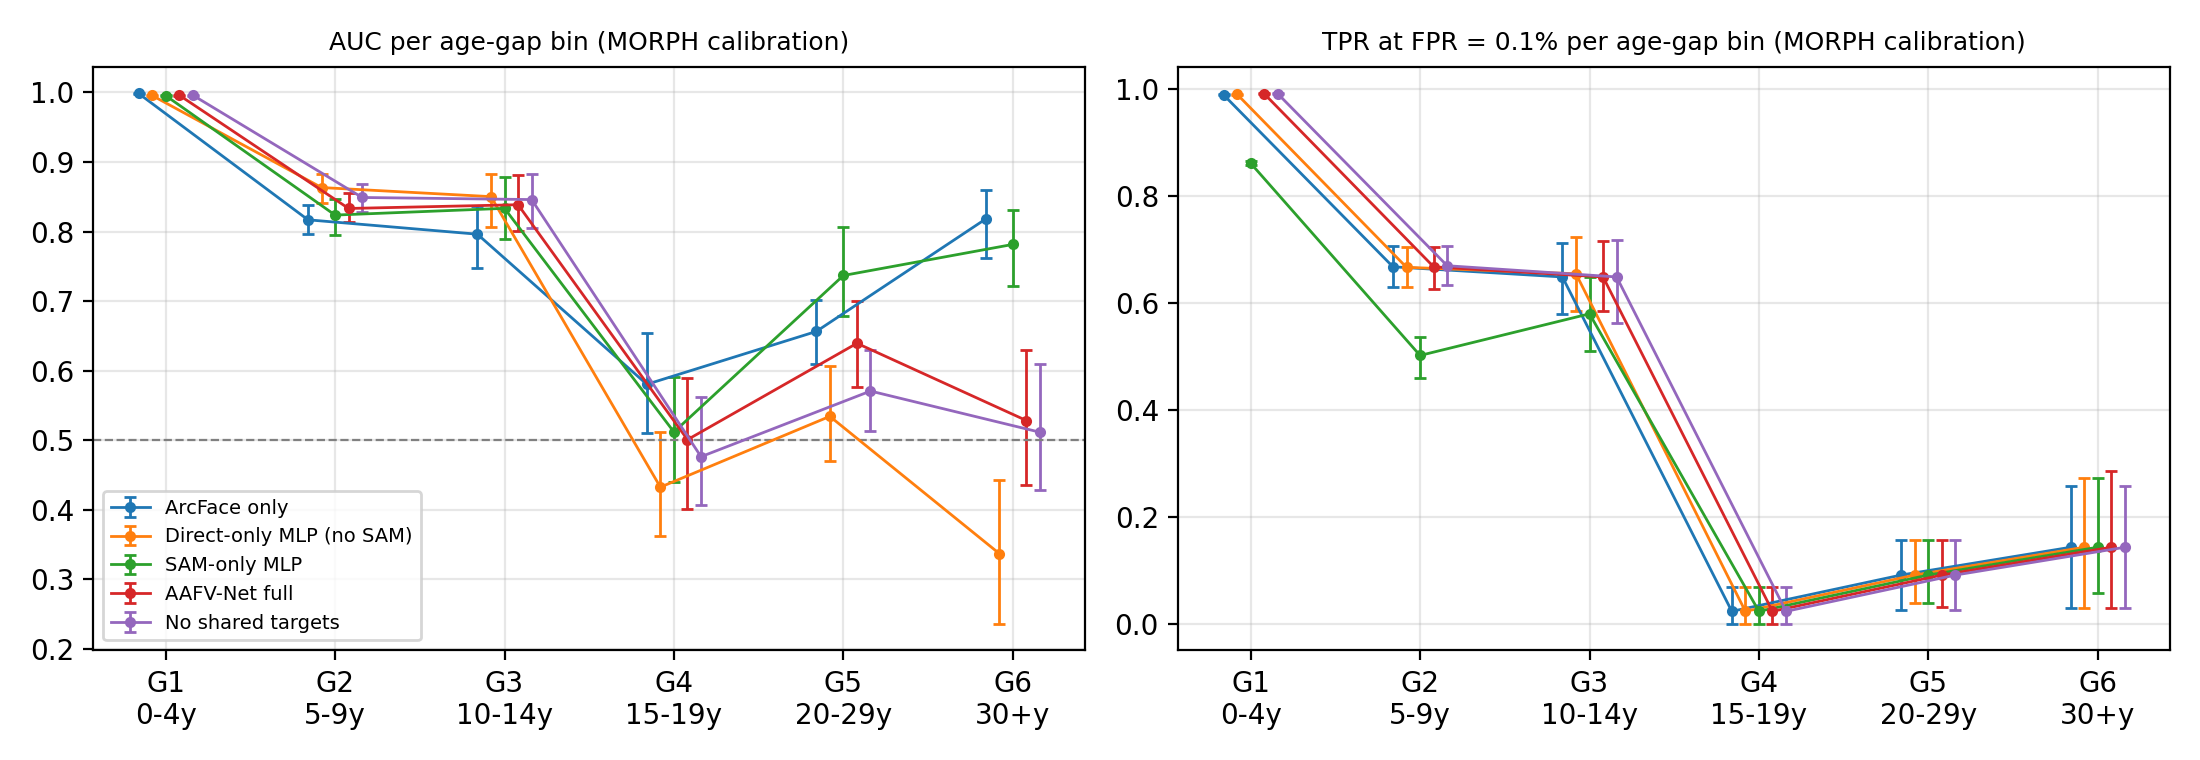
\includegraphics[width=\linewidth]{figures/fig_gap_ranking.png}
\caption{Ranking quality per age-gap bin on the MORPH calibration split for five variants (95\% intervals from the original pipeline). Left: AUC. Right: TAR at FPR $=10^{-3}$. Bins of 15 years and more are analysed in Section~\ref{sec:labels}.}
\label{fig:gap}
\end{figure}

\subsection{Generated faces add no evidence at matched operating points}
\label{sec:generated}
Table~\ref{tab:matched} compares, on identical pairs, ArcFace on the original pair, ArcFace on the generated pairs (the score entering the SAM branch), the fused AAFV-Net score, and a person-cross-fitted logistic regression on the two ArcFace scores. Against random impostors the generated-pair score is significantly weaker than the original-pair score at 0--4 years ($\Delta$TAR $=-0.076$) and 5--9 years ($-0.072$), and combining the two changes TAR by exactly zero in every bin. At 5--9 years the generated-pair score has a nominally higher AUC ($+0.043$, 95\% CI $[0.000, 0.106]$), but this does not survive at the low false-match rates where decisions are made, and the combined score's AUC is not higher ($-0.026$, $[-0.065, +0.003]$). The fused score is slightly below ArcFace at 0--4 years ($-0.002$, $[-0.004,-0.001]$).

\begin{table}[t]
\centering
\caption{Per-pair comparison at matched false-match rate (FMR $=10^{-3}$) on the MORPH calibration split. $\Delta$ is the difference in TAR from ArcFace on the original pair, with a 95\% paired two-way person-cluster bootstrap interval (300 replicates). For gaps of 15 years and more every score has the same TAR against random impostors (15--19 y: 0.023 (n=44); 20--29 y: 0.091 (n=77); 30+ y: 0.143 (n=35)); those bins are analysed in Section~\ref{sec:labels}.}
\label{tab:matched}
\footnotesize
\setlength{\tabcolsep}{3pt}
\fittab{\begin{tabular}{@{}llccc@{}}
\toprule
Gap, y ($n$ gen.) & Score & TAR & $\Delta$TAR [95\% CI] & AUC \\
\midrule
\multicolumn{5}{@{}l}{\emph{Random impostors}} \\
0--4 (22914) & ArcFace (original pair) & 0.996 & -- & 0.999 \\
 & ArcFace (generated pair) & 0.920 & -0.076 [-0.112, -0.051] & 0.999 \\
 & AAFV-Net fused & 0.994 & -0.002 [-0.004, -0.001] & 0.996 \\
 & LogReg: original $+$ generated & 0.996 & +0.000 [+0.000, +0.000] & 0.999 \\
\addlinespace[1pt]
5--9 (594) & ArcFace (original pair) & 0.682 & -- & 0.840 \\
 & ArcFace (generated pair) & 0.609 & -0.072 [-0.111, -0.032] & 0.883 \\
 & AAFV-Net fused & 0.668 & -0.013 [-0.024, +0.000] & 0.807 \\
 & LogReg: original $+$ generated & 0.682 & +0.000 [+0.000, +0.000] & 0.814 \\
\addlinespace[1pt]
10--14 (174) & ArcFace (original pair) & 0.655 & -- & 0.813 \\
 & ArcFace (generated pair) & 0.644 & -0.011 [-0.045, +0.000] & 0.766 \\
 & AAFV-Net fused & 0.649 & -0.006 [-0.024, +0.000] & 0.821 \\
 & LogReg: original $+$ generated & 0.655 & +0.000 [+0.000, +0.000] & 0.806 \\
\addlinespace[1pt]
\multicolumn{5}{@{}l}{\emph{ArcFace-mined look-alikes}} \\
0--4 (22914) & ArcFace (original pair) & 0.985 & -- & 0.996 \\
 & ArcFace (generated pair) & 0.391 & -0.594 [-0.689, -0.513] & 0.974 \\
 & AAFV-Net fused & 0.988 & +0.003 [+0.001, +0.006] & 0.998 \\
 & LogReg: original $+$ generated & 0.981 & -0.004 [-0.006, -0.001] & 0.996 \\
\addlinespace[1pt]
5--9 (594) & ArcFace (original pair) & 0.653 & -- & 0.682 \\
 & ArcFace (generated pair) & 0.293 & -0.360 [-0.559, -0.117] & 0.683 \\
 & AAFV-Net fused & 0.653 & +0.000 [-0.012, +0.014] & 0.988 \\
 & LogReg: original $+$ generated & 0.653 & +0.000 [-0.012, +0.013] & 0.683 \\
\addlinespace[1pt]
10--14 (174) & ArcFace (original pair) & 0.649 & -- & 0.655 \\
 & ArcFace (generated pair) & 0.397 & -0.253 [-0.479, -0.059] & 0.647 \\
 & AAFV-Net fused & 0.649 & +0.000 [+0.000, +0.355] & 0.992 \\
 & LogReg: original $+$ generated & 0.649 & +0.000 [+0.000, +0.000] & 0.655 \\
\addlinespace[1pt]
\bottomrule
\end{tabular}}
\end{table}


\begin{figure}[t]
\centering
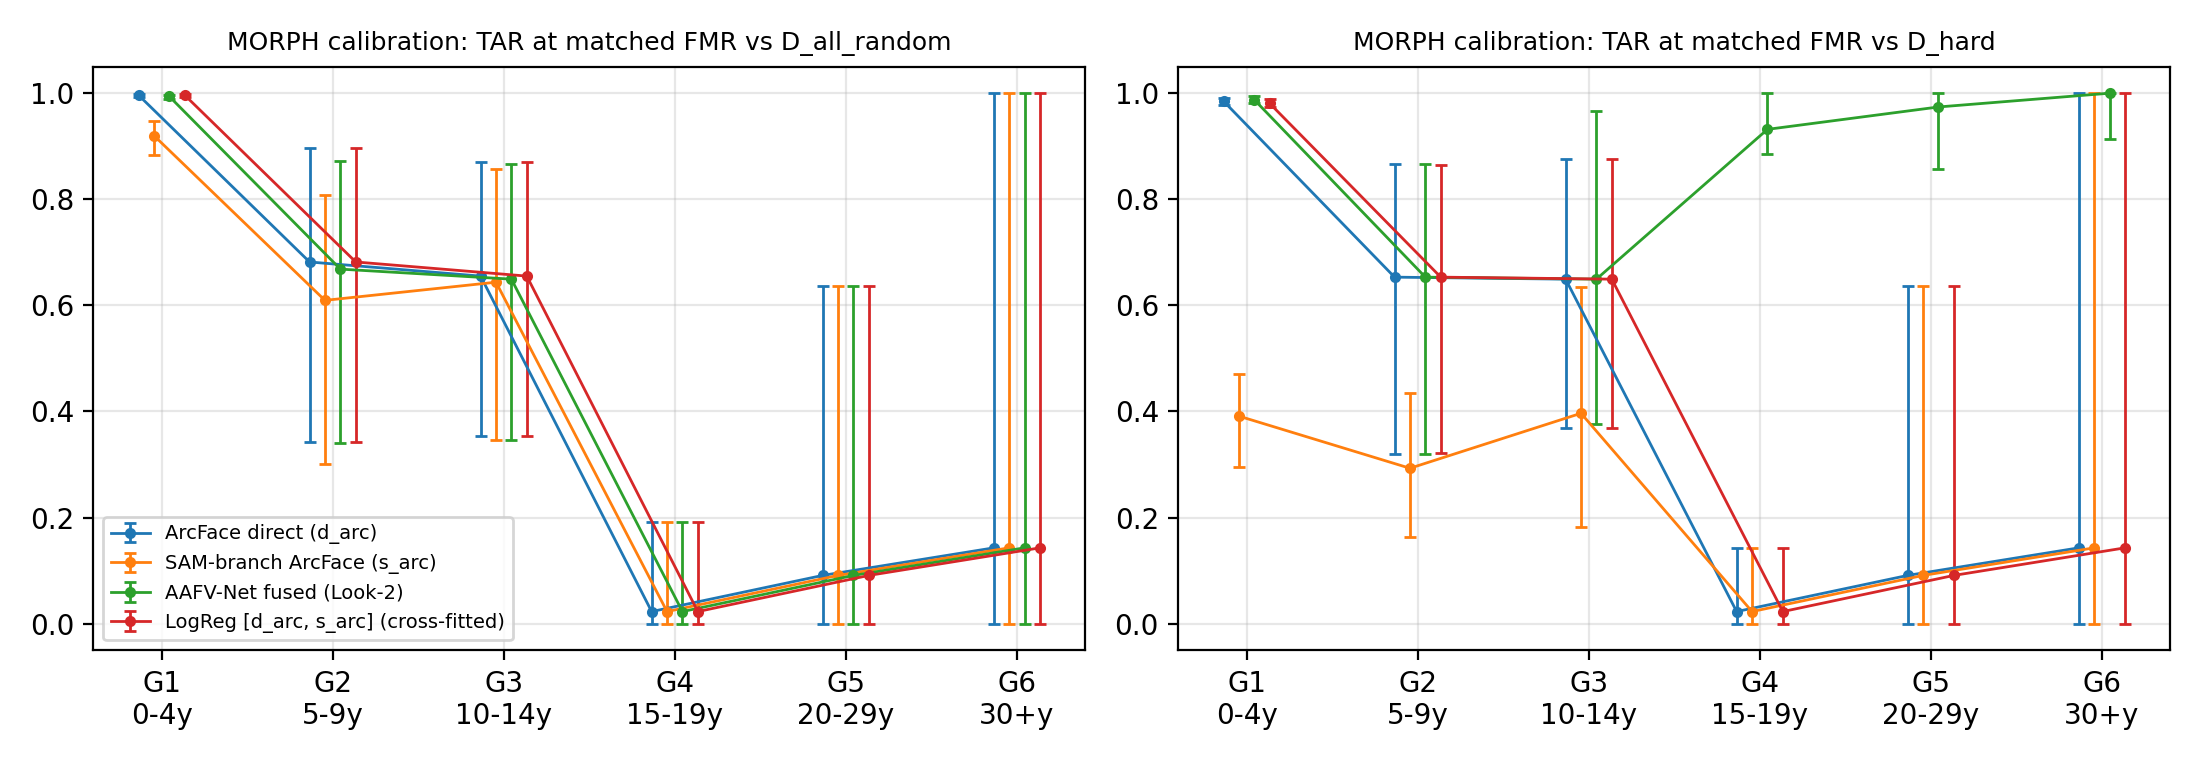
\includegraphics[width=\linewidth]{figures/fig_matched_fmr.png}
\caption{TAR at matched FMR per gap bin on the MORPH calibration split for the four scores of Table~\ref{tab:matched}, against random impostors (left) and ArcFace-mined look-alikes (right); 95\% person-cluster bootstrap intervals.}
\label{fig:matched}
\end{figure}

Against ArcFace-mined look-alikes the fused score gains $+0.003$ at 0--4 years, while the generated-pair score alone is much weaker (TAR 0.391 versus 0.985) and the two-score combination is not better than ArcFace. The fused system's strong look-alike rejection reported earlier therefore does not come from the generated evidence. It is shared by a direct-only variant without any SAM input (Table~\ref{tab:decision}: TPR 0.971 versus 0.973) and is consistent with half of the training negatives having been mined in the same way, which places $\mathcal{D}_\mathrm{hard}$ in the training distribution. The very large gains at 15 years and more in Fig.~\ref{fig:matched} (right) arise because the fused network scores mined look-alikes below even the mislabelled ``genuine'' pairs described in Section~\ref{sec:labels}; they are not evidence of long-gap capability.

\subsection{What the fusion network learned}
\label{sec:probe}
Table~\ref{tab:probe} inspects the frozen network. The original-pair head places almost all of its weight on ArcFace; EfficientNet, VGG-Face, LPIPS and SSIM receive weights an order of magnitude smaller. Moving the original-pair logit across its plausible range changes the fused logit about six times more than moving the generated-pair logit, and the response to the generated-pair logit and to $R_\mathrm{sam}$ is no larger than that of variants trained with those inputs held constant, whose response is arbitrary. Gap and quality are used modestly. The fused score is, in effect, a monotone transform of ArcFace with small context-dependent offsets---which explains Sections~\ref{sec:decision} and~\ref{sec:generated}.

\begin{table}[t]
\centering
\caption{What the frozen fusion network uses. Top: weights of the two linear branch heads on the five z-scored similarities (mean of 3 seeds). Bottom: change of the fused logit when one input moves across a plausible range (branch logits: bias $\pm 3\|w\|$; gap 5$\to$25 y; quality 0.3$\to$0.9; $R_\mathrm{sam}$ 0.2$\to$0.9). Untrained controls are variants trained with that input held constant, whose response is arbitrary.}
\label{tab:probe}
\footnotesize
\setlength{\tabcolsep}{4pt}
\fittab{\begin{tabular}{@{}lccccc@{}}
\toprule
Head & ArcFace & EfficientNet & VGG-Face & LPIPS & SSIM \\
\midrule
Original pair & -0.255 & +0.005 & -0.011 & +0.016 & -0.010 \\
Generated pairs & -0.101 & +0.149 & -0.057 & -0.004 & +0.023 \\
\bottomrule
\end{tabular}}

\vspace{4pt}
\fittab{\begin{tabular}{@{}lcc@{}}
\toprule
Input & Swing (full model) & Untrained control \\
\midrule
Original-pair branch logit & 25.1 & -- \\
Generated-pair branch logit & 4.1 & 4.4 (direct-only) \\
Synthesis reliability $R_\mathrm{sam}$ & 0.40 & 0.51 (no context) \\
Age gap & 0.90 & 0.23 (no context) \\
Image quality & 0.87 & 0.26 (no context) \\
\bottomrule
\end{tabular}}
\end{table}


\subsection{Integrity of the calibration procedure}
\label{sec:integrity}
The calibration code supported two post-hoc steps after inspecting a contact sheet of the highest-scoring calibration impostors: relabelling pairs and quarantining additional persons. The run logs show that the draft calibration of the original (five-network) model reached $T_\mathrm{acc}=1.0129$ at $\rho=0.20$, admitting nobody; the highest-scoring impostors were two pairs of persons with fused probabilities of 0.996 and 0.961. Of the 858 quarantined persons, 854 are explained by the automatic duplicate rule; the remaining four are exactly these two pairs. Restoring their 932 pairs (16 genuine, 4 person-disjoint random, 112 mined, 800 repeated random) raises $T_\mathrm{acc}$ above 1 and reduces genuine acceptance to 0\% for every value of $\rho$ (Table~\ref{tab:reconstruction}, bottom). Every acceptance rate reported for the system---73.26\% on calibration, 79.74\% and 70.07\% on the two test looks---depends on this removal. The images would be needed to decide whether the four are duplicate records of two people or genuine look-alikes; in either case the step was taken after the scores were seen and must be reported.

The zero-failure bounds reported in earlier drafts are arithmetically correct (Table~\ref{tab:stats}), but they describe two different statements---a calibration-side certificate and a held-out audit, each with or without a multiplicity correction---and every method in Table~\ref{tab:decision}, including plain ArcFace, attains the same values, because all of them observe no random-impostor false accept. The calibration certificate further assumes that the scorer was fixed independently of the calibration impostors; the split was used to develop guards, variants and the floor $\rho$, and identities were removed after their scores were seen. We therefore do not regard these bounds as evidence about the method.

\begin{table}[t]
\centering
\caption{The zero-failure upper bounds $\varepsilon = 1-\delta^{1/n}$ on random-impostor FAR that appeared in earlier versions, recomputed. All are arithmetically correct; they describe two different statements (a calibration-side certificate and a held-out audit), and every method in Table~\ref{tab:decision} attains the same values.}
\label{tab:stats}
\footnotesize
\fittab{\begin{tabular}{@{}lccc@{}}
\toprule
Statement & $n$ & $\delta$ & $\varepsilon$ (\%) \\
\midrule
Calibration certificate & 1{,}170 & 0.05 & 0.256 \\
Calibration certificate, union over 3 values of $\rho$ & 1{,}170 & $0.05/3$ & 0.349 \\
Held-out audit, one look & 1{,}149 & 0.05 & 0.260 \\
Held-out audit, Bonferroni over 2 looks & 1{,}149 & 0.025 & 0.321 \\
\bottomrule
\end{tabular}}
\end{table}


\subsection{MORPH long-gap labels}
\label{sec:labels}
Every method reaches chance-level AUC at 15--19 years (Fig.~\ref{fig:gap}), which is implausible for modern recognizers on true adult pairs. Table~\ref{tab:labels} shows why. MORPH file names encode the subject's sex; within calibration ``same-person'' pairs the two names record different sexes in 0.0\% of pairs at 0--4 years but in 18--29\% at 15 years and more. Pairs whose file identifiers differ (a consequence of merging records with truncated or suffix-sharing identifiers into one person) are impostor-like far more often than pairs with matching identifiers at 5--14 years (58--80\% versus 5--8\%). On the test split, an independently trained Siamese ViT and the fused system find the same genuine pairs impostor-like (97\% at 15--19 years for both). The merge was correct for most short-gap pairs, which is why the problem went unnoticed; at long gaps it links different people, whose arbitrary age differences then appear as long gaps. As processed, MORPH contains essentially no valid long-gap genuine pairs, and the long-gap ``collapse'' reported for this system describes label errors rather than aging.

\begin{table*}[t]
\centering
\caption{Integrity of MORPH ``same-person'' pairs as processed by the pipeline. Sex mismatch: the sex letters encoded in the two file names differ. Impostor-like: the pair scores below the 99th percentile of random impostors in the same gap bin. Calibration columns use the direct ArcFace score; test columns are a post-hoc reading of logged outputs of the fused system (Look~1) and of an independently trained Siamese ViT.}
\label{tab:labels}
\footnotesize
\fittab{\begin{tabular}{@{}lccccccc@{}}
\toprule
 & \multicolumn{5}{c}{Calibration split} & \multicolumn{2}{c}{Test split (post hoc)} \\
\cmidrule(lr){2-6}\cmidrule(l){7-8}
Gap (y) & $n$ & Sex mismatch (\%) & File ids differ (\%) & Impostor-like (\%) & Impostor-like: ids differ / same (\%) & $n$ & Impostor-like: fused / ViT (\%) \\
\midrule
0--4 & 22,914 & 0.0 & 27.5 & 0.2 & 0.8 / 0.0 & 23631 & 0.4 / 4.3 \\
5--9 & 594 & 1.9 & 49.7 & 31.5 & 58.3 / 5.0 & 266 & 13.9 / 20.3 \\
10--14 & 174 & 2.9 & 36.8 & 34.5 & 79.7 / 8.2 & 184 & 23.9 / 23.9 \\
15--19 & 44 & 20.5 & 79.5 & 97.7 & 97.1 / 100.0 & 75 & 97.3 / 97.3 \\
20--29 & 77 & 18.2 & 77.9 & 90.9 & 96.7 / 70.6 & 137 & 94.9 / 97.8 \\
30+ & 35 & 28.6 & 65.7 & 85.7 & 91.3 / 75.0 & 12 & 0.0 / 0.0 \\
\bottomrule
\end{tabular}}
\end{table*}


\subsection{How the generator changes faces}
Table~\ref{tab:sam} and Fig.~\ref{fig:sam} summarise all 379,930 SAM outputs. Similarity to the source falls from a median of 0.51 for shifts under 5 years to 0.35 for aging by 30 years or more, when 23\% of outputs fall below 0.30; aging degrades identity more than rejuvenation at large shifts, and age accuracy worsens from about 2 to about 5 years. These values come from the recognizer inside the pipeline, fed resized crops, so they describe the generator only relative to that recognizer; even a shift of a few years reduces the similarity to about 0.5, indicating that the generator rewrites the face substantially at every target age.

\begin{table}[t]
\centering
\caption{Identity similarity of SAM-generated faces to their source image (ArcFace cosine) and age accuracy, by direction and size of the age shift. ArcFace is the recognizer used inside AAFV-Net and received resized FFHQ crops, so these values are descriptive, not an independent identity test.}
\label{tab:sam}
\footnotesize
\setlength{\tabcolsep}{3pt}
\fittab{\begin{tabular}{@{}lcrcccc@{}}
\toprule
Direction & $|$shift$|$ (y) & $n$ & Median cos & 10th pct & $<0.30$ (\%) & Age error (y) \\
\midrule
older & 0--4 & 46,930 & 0.508 & 0.413 & 0.3 & 2.2 \\
older & 5--14 & 80,657 & 0.485 & 0.387 & 0.8 & 2.9 \\
older & 15--29 & 64,935 & 0.426 & 0.324 & 5.7 & 3.8 \\
older & 30+ & 12,613 & 0.352 & 0.261 & 23.1 & 4.8 \\
younger & 0--4 & 47,789 & 0.513 & 0.417 & 0.3 & 2.4 \\
younger & 5--14 & 77,512 & 0.500 & 0.402 & 0.6 & 3.2 \\
younger & 15--29 & 41,444 & 0.460 & 0.359 & 2.3 & 3.8 \\
younger & 30+ & 8,050 & 0.395 & 0.292 & 11.9 & 4.0 \\
\bottomrule
\end{tabular}}
\end{table}


\begin{figure}[t]
\centering
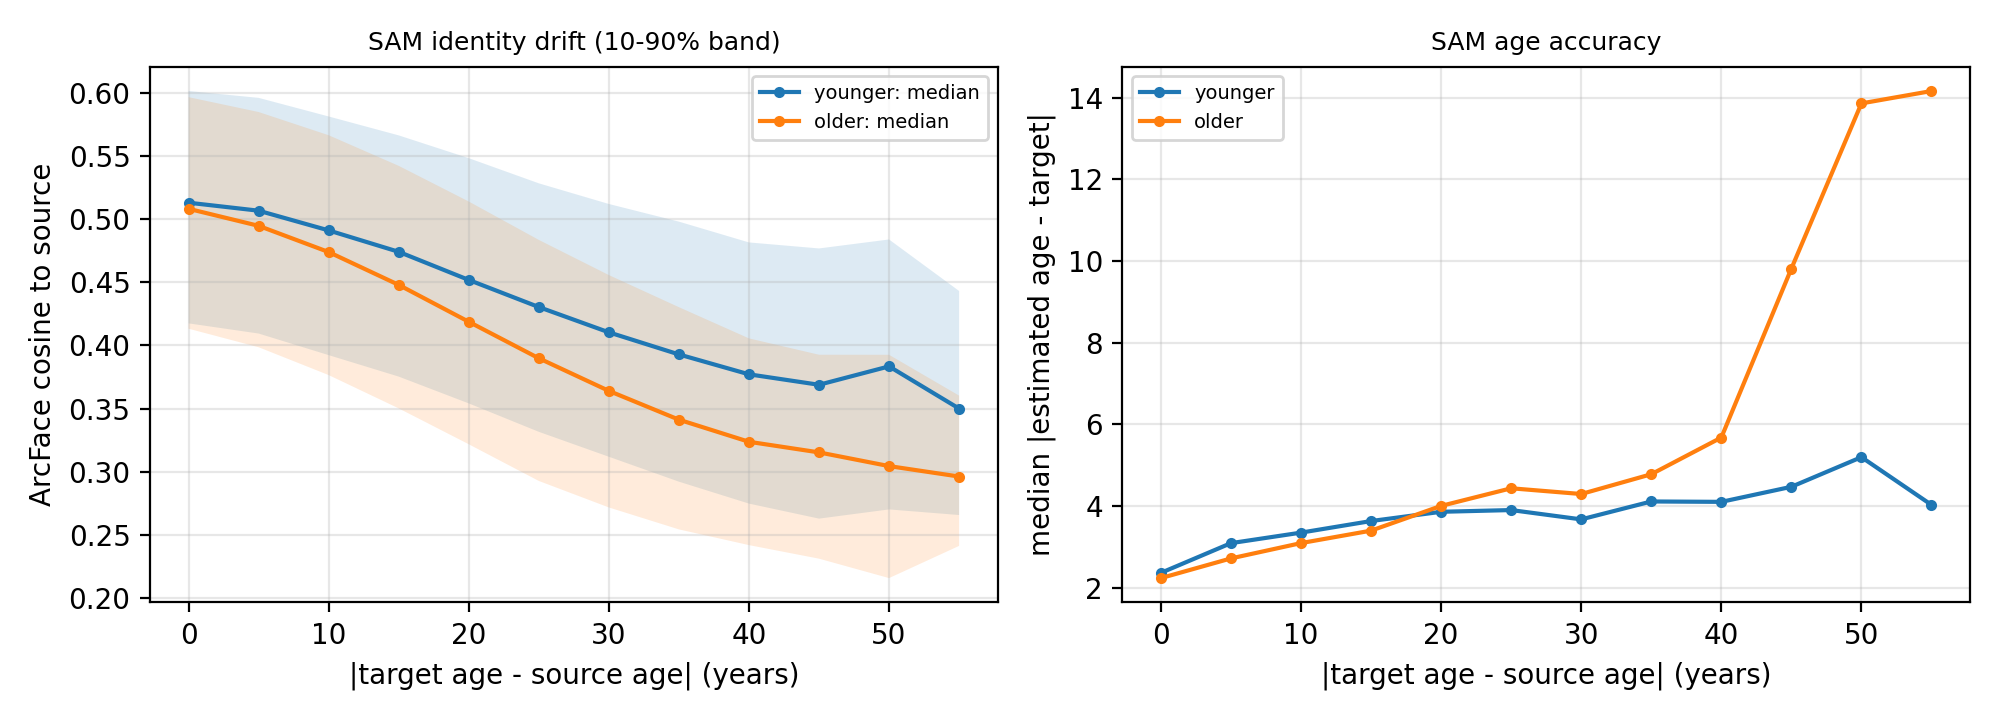
\includegraphics[width=\linewidth]{figures/fig_sam_drift.png}
\caption{SAM outputs: ArcFace similarity to the source (median, 10--90\% band) and median age error, by size of the age shift and direction.}
\label{fig:sam}
\end{figure}

\subsection{External data}
On FG-NET adults, the earlier drafts reported that AAFV-Net auto-accepted 51.92\% of genuine pairs against 40.38\% for ArcFace, but falsely rejected 18.20\% against a 1\% target; on all ages it made four false accepts in 20,000 impostor pairs, all involving children aged 0--4 with fused probabilities of 0.966--1.000. No per-pair FG-NET scores were logged for the fused system or ArcFace, so a matched-FMR comparison on FG-NET is not possible from the recovered data.

\section{A Protocol for the Open Question}
\label{sec:protocol}
Our results show that, in this system and on MORPH, generated faces add no verification evidence; they do not show that generated faces \emph{cannot} help at genuine long gaps, because MORPH has none and the identity measurements above use the recognizer inside the pipeline. We have therefore pre-registered a test before running it. It uses AgeDB~\cite{moschoglou2017agedb} and FG-NET~\cite{lanitis2002fgnet}; person-disjoint folds with all pairs formed within a fold; impostors formed by replacing the older image with a different person of matched age and sex, so that the younger image is progressed by the same generator call for genuine and impostor pairs; recognizers outside the pipeline (AdaFace~\cite{kim2022adaface} and MagFace~\cite{meng2021magface}, with standard five-point alignment); two generators (SAM~\cite{alaluf2021sam} and FADING~\cite{chen2023fading}); a person-cross-fitted combination of original and generated scores; and an age-only control in which each generated face is replaced by a different person's face generated at the same target age. The decision criterion is a gain in TAR at FMR $10^{-3}$ in the 15--29 or 30+ year adult bins whose Bonferroni-adjusted interval excludes zero, with no gain under the control. The full pre-registration and tested code are part of the supplementary material. Only if this test is positive is a method that learns from generated faces worth building.

\section{Discussion and Limitations}
\textbf{What generalises.} Three lessons extend beyond this system. First, comparisons of selective verifiers must be made at matched false-match rates and matched review workload; a decision layer can create or hide large differences in automation between methods that discriminate identically. Second, synthetic evidence should be tested per pair against the recognizer it is meant to help, with a combination model fitted out of sample; aggregate system results cannot separate its contribution. Third, longitudinal datasets need linkage audits before long-gap claims: the errors here are concentrated exactly where the scientific claim lives.

\textbf{Limitations.} All controlled comparisons use the MORPH calibration split, which was also used during the development of AAFV-Net; they are re-analyses of a fixed model, not new confirmatory evaluations. The identity measurements use the pipeline's own recognizer with non-standard alignment. The label analysis relies on file names and scores; a visual audit of a sample of long-gap pairs is needed to estimate the error rate precisely. Whether the four removed identities are duplicates is unresolved. FG-NET results could not be re-analysed. The test-split readings are post hoc.

\section{Conclusion}
Re-examined at matched operating points, AAFV-Net's synthetic age-progression branch contributes no verification evidence beyond ArcFace on MORPH, its acceptance deficit is a property of its decision layer, its published operating point depends on a post-hoc calibration exclusion, and the long-gap MORPH pairs on which age-related conclusions would rest are largely mislabelled. Whether generated faces can help at genuine long gaps remains open; we provide a pre-registered protocol to test it.

\section*{Data and Code Availability}
MORPH and FG-NET are available from their providers under licence; no images are redistributed. Analysis scripts, aggregate result tables, the hash manifest of the frozen models and the pre-registered protocol are available from the authors [repository to be confirmed].

\section*{Ethics Statement}
This study uses existing, licensed face datasets and creates no new data from human participants. [Institutional review status to be confirmed by the authors.] The datasets contain arrest photographs with a skewed demographic composition; results should not be generalised to other populations, and long-term face matching carries surveillance risks that deployments must address.

\section*{Use of AI Tools}
An AI assistant (Claude, Anthropic) was used to write and verify the analysis code, to check references against their sources, and to draft this manuscript under the authors' direction. All reported numbers are produced by the scripts listed in the supplementary material and were checked against their sources. The authors are responsible for the content. [To be revised and confirmed by the authors before submission.]

\bibliographystyle{IEEEtran}
\bibliography{references}

\end{document}
